\section[Architectural Design]{\hyperlink{toc}{Architectural Design}}
	\label{sec:architecturalDesign}
	
	In the following section we describe precisely the architecture of our system. Starting with the highest possible view we first give an illustration of all the systems that SafeStreets is going to interact with. Differently than how we did in the RASD \cite{RASD} document here we need to precise which are the systems that provide the interfaces already mentioned in order to obtain a clear description of the communication between each system and the one we are designing.\\
	
	After the first global description we start focusing on the system, first with a clear listing of all the components needed to obtain the functionalities of the application and then with their deployment (\ref{sec:deploymentDiagram}) and runtime (\ref{sec:runtimeView}) utilization.\\
	
	The section concludes first with the precise definition of the architectural patterns used to deploy all the components identified and finally with other design decisions (\ref{sec:otherDesignDecisions}) that have been chosen in the architectural design process.	
	
	\subsection[Overview]{\hyperlink{toc}{Overview}}
		\label{sec:overview}
		
		\subsubsection[General Context]{\hyperlink{toc}{General Context}}
			\label{sec:generalContext}
			
			Let's start this huge and dense section with the highest level of visibility possible of our system in order to first understand which are the other system it needs to interact with. SafeStreets is a crowd-sourced application that intends to provide services to two typologies of customers: \textbf{users} and \textbf{authorities}. Hence the crowd is composed by the users who provide the system information thanks to the core functionality offered that is the \emph{notification of a traffic violation}.\\
			
			To understand which systems are involved in each of the functionalities offered by SafeStreets that will now be called as already mentioned in the RASD document \cite{RASD}:
			
			\begin{itemize}
				\item \textbf{Access Functionality:} service that allows customers to register to the system in order to be recognized
				\item \textbf{Core Functionality:} service provided only to the users to allow them to notify a traffic violation.
				\item \textbf{Basic Functionalities:} mining services over the information provided by the users redistributed to the customers with different levels of visibility.
				\item \textbf{Advanced Functionalities:} services that provide the safety of an area chosen by the customers and some suggestions for possible interventions for the streets that are found to be dangerous.
			\end{itemize}
		
			In the following picture we illustrate the \textbf{context viewpoint} (\autoref{fig:contextViewpoint}) as we can later describe how each of the systems identified are needed in order to obtain the functionalities just presented.
			
			\newpage
			
			\begin{figure}[ht]
				\centering
				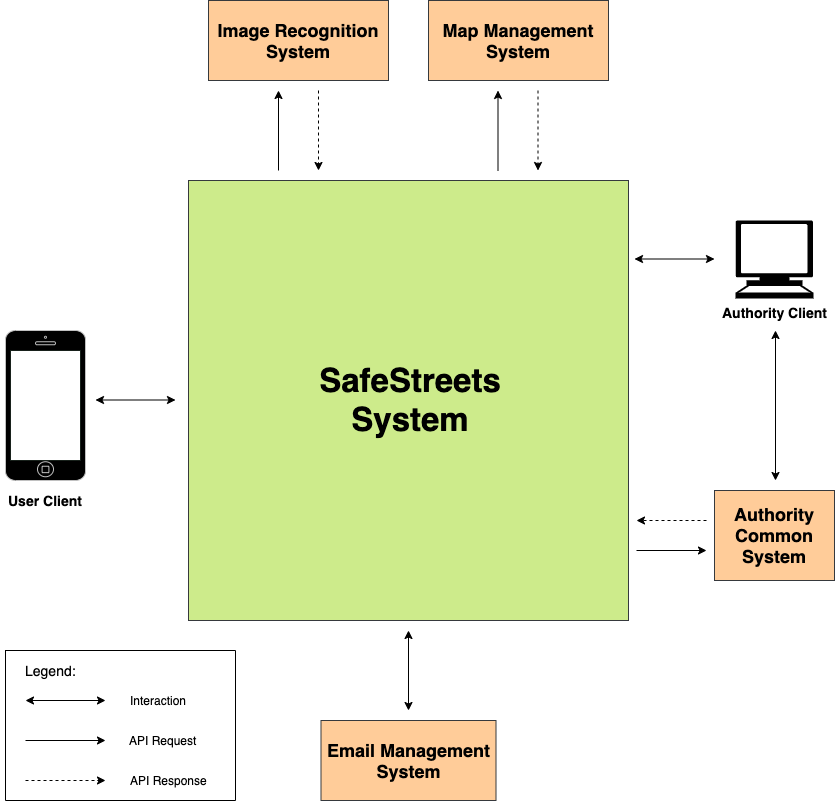
\includegraphics[scale=0.4]{contextViewPoint.png}
				\caption{\label{fig:contextViewpoint} Context Viewpoint}
			\end{figure}
		
			Now that we know which are the systems that needed, before seeing which are the modules that will consider the communication with each of them let's understand first for which functionality they are used for. The following table lists the three types of functionalities and a tick (\xtick) is used to express that the functionality needs the external systems services in order to be realized.
			
			\begin{center}
				\scalebox{0.7}{
					\begin{tabular}{|c|c|c|c|c|}
						\hline
						\diagbox{\textbf{Functionality}}{\textbf{System}} & Image Recognition & Map Management & Email Management & Authority Common \\ \hline
						Access & & & \xtick & \\ \hline
						Core & \xtick & \xtick & & \\ \hline
						Basic & & \xtick & & \\ \hline
						Advanced & & \xtick & & \xtick \\ \hline
					\end{tabular}
				} \captionof{table}{\label{tab:functionalityTable} System Mapping Table}
			\end{center}
		
		\subsubsection[Composition Diagram]{\hyperlink{toc}{Composition Diagram}}
			\label{sec:compositionDiagram}
			
			With the definition of the systems used by SafeStreets we are now able to highlight the modules used by our system in order to benefit of their services. In the following diagram we divide the system in three different types of areas, each one containing the modules considered critical for that competence.
			
			\newpage
			
			\begin{figure}[ht]
				\centering
				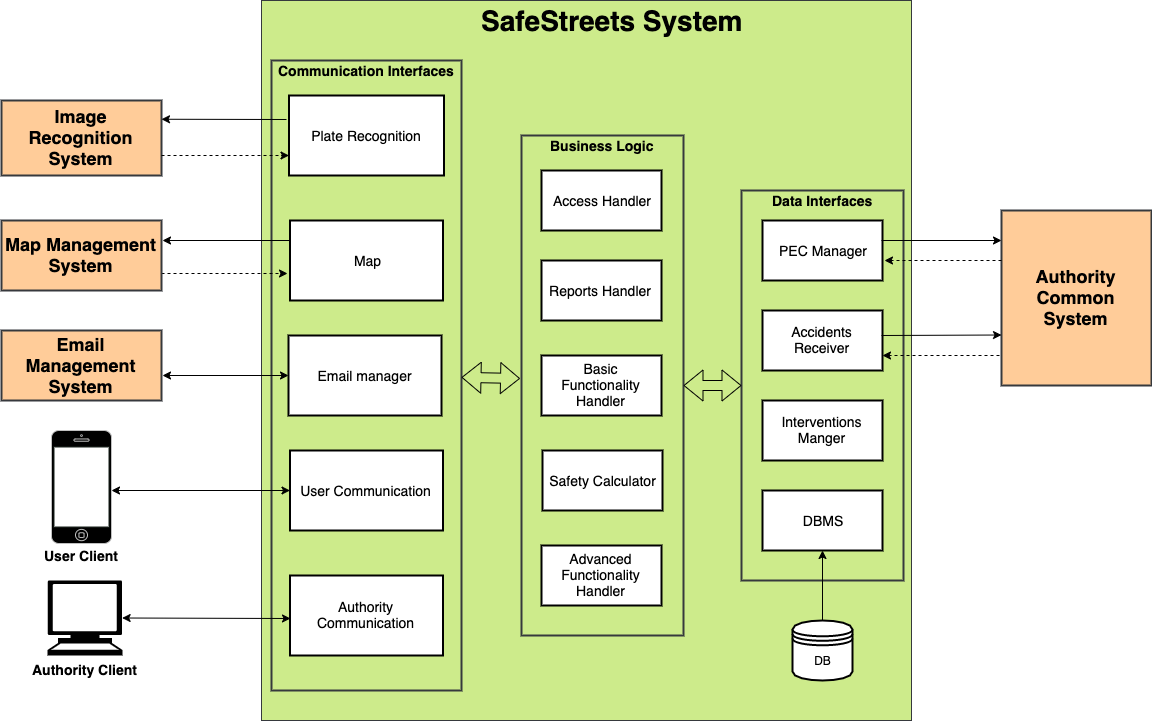
\includegraphics[scale=0.3]{compositionViewPoint.png}
				\caption{\label{fig:compositionDiagram} Composition Diagram}
			\end{figure}
		
			As we see can see in the picture above, the system is composed of three areas, each one specialized on a particular behaviors.
			
			\paragraph{Communication Interfaces} Are the interfaces that allows our system to interact with externally active agents or systems that provide services needed by the business logic. In fact, as we notice in the left hand-side of the diagram we have:
			
			\begin{itemize}
				\item \textbf{Image Recognition System:} provides thanks to an interface the methods to deal with the recognition of the plate of the vehicles
				\item \textbf{Map Management System:} provides thanks to an interface the methods to deal with all the issues related to the geographical positioning and map interaction
				\item \textbf{Email Management System:} provides the minimal email services that SafeStreets needs to consider in order to provide the recovery of the credentials and more important the recognition of the authorities
				\item \textbf{User Client:} is the client used by a user in order to benefit of SafeStreets functionalities
				\item \textbf{Authority Client:} is the client used by an authority in order to benefit of SafeStreets functionalities
			\end{itemize}
		
			All the modules defined here will bring inside the system all the services and requests coming from the outside as the ones in the business modules can process them and provide the functionalities of SafeStreets
			
			\paragraph{Business Logic} Now we have the modules that are thought to deal with the functionalities that the system has to provide. As we can see also in this case, we have a correspondence between the functionalities described in the previous section and the modules now listed:
			
			\begin{itemize}
				\item Access Handler
				\item Reports Handler
				\item Basic Functionality Handler
				\item Safety Calculator
				\item Advanced Functionality Handler
			\end{itemize}
		
			\paragraph{Data Interfaces} These last interface instead are separated from the initial ones because they provide a way to the system to access external data he needs to use in order to provide its functionalities. As we can see in the right hand-side of the diagram we only have the \textbf{Authority Common Interface} that provides the methods to retrieve all the data of the accidents that took place in a certain city and the list of all the PEC addresses of the authorities.
			
			\newpage
		
	\subsection[Component View]{\hyperlink{toc}{Component View}}
		\label{sec:componentView}
		
		\begin{figure}[ht]
			\centering
			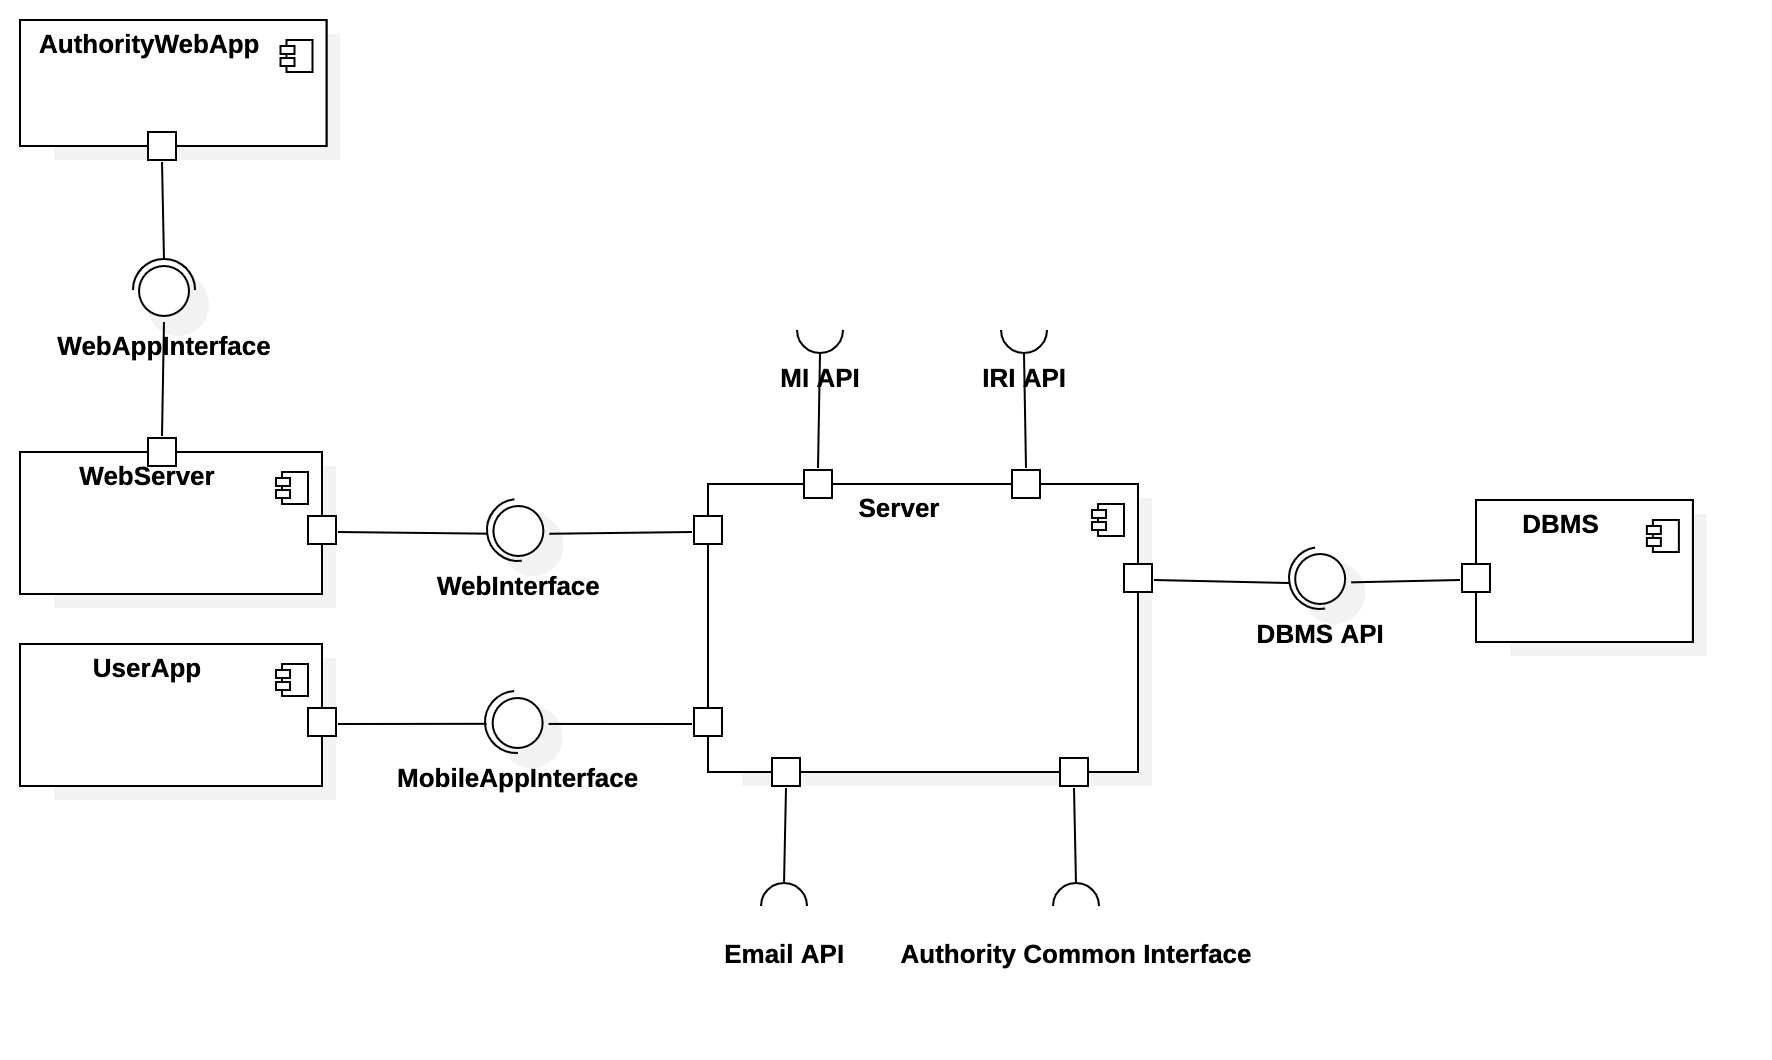
\includegraphics[scale=0.2]{/diagrams/components/highLevel.png}
			\caption{\label{fig:highLevelComp} High Level Component Diagram}
		\end{figure}
	
		\subsubsection[Server Component]{\hyperlink{toc}{Server Component}}
			\label{sec:serverComponent}
			
			\begin{figure}[ht]
				\centering
				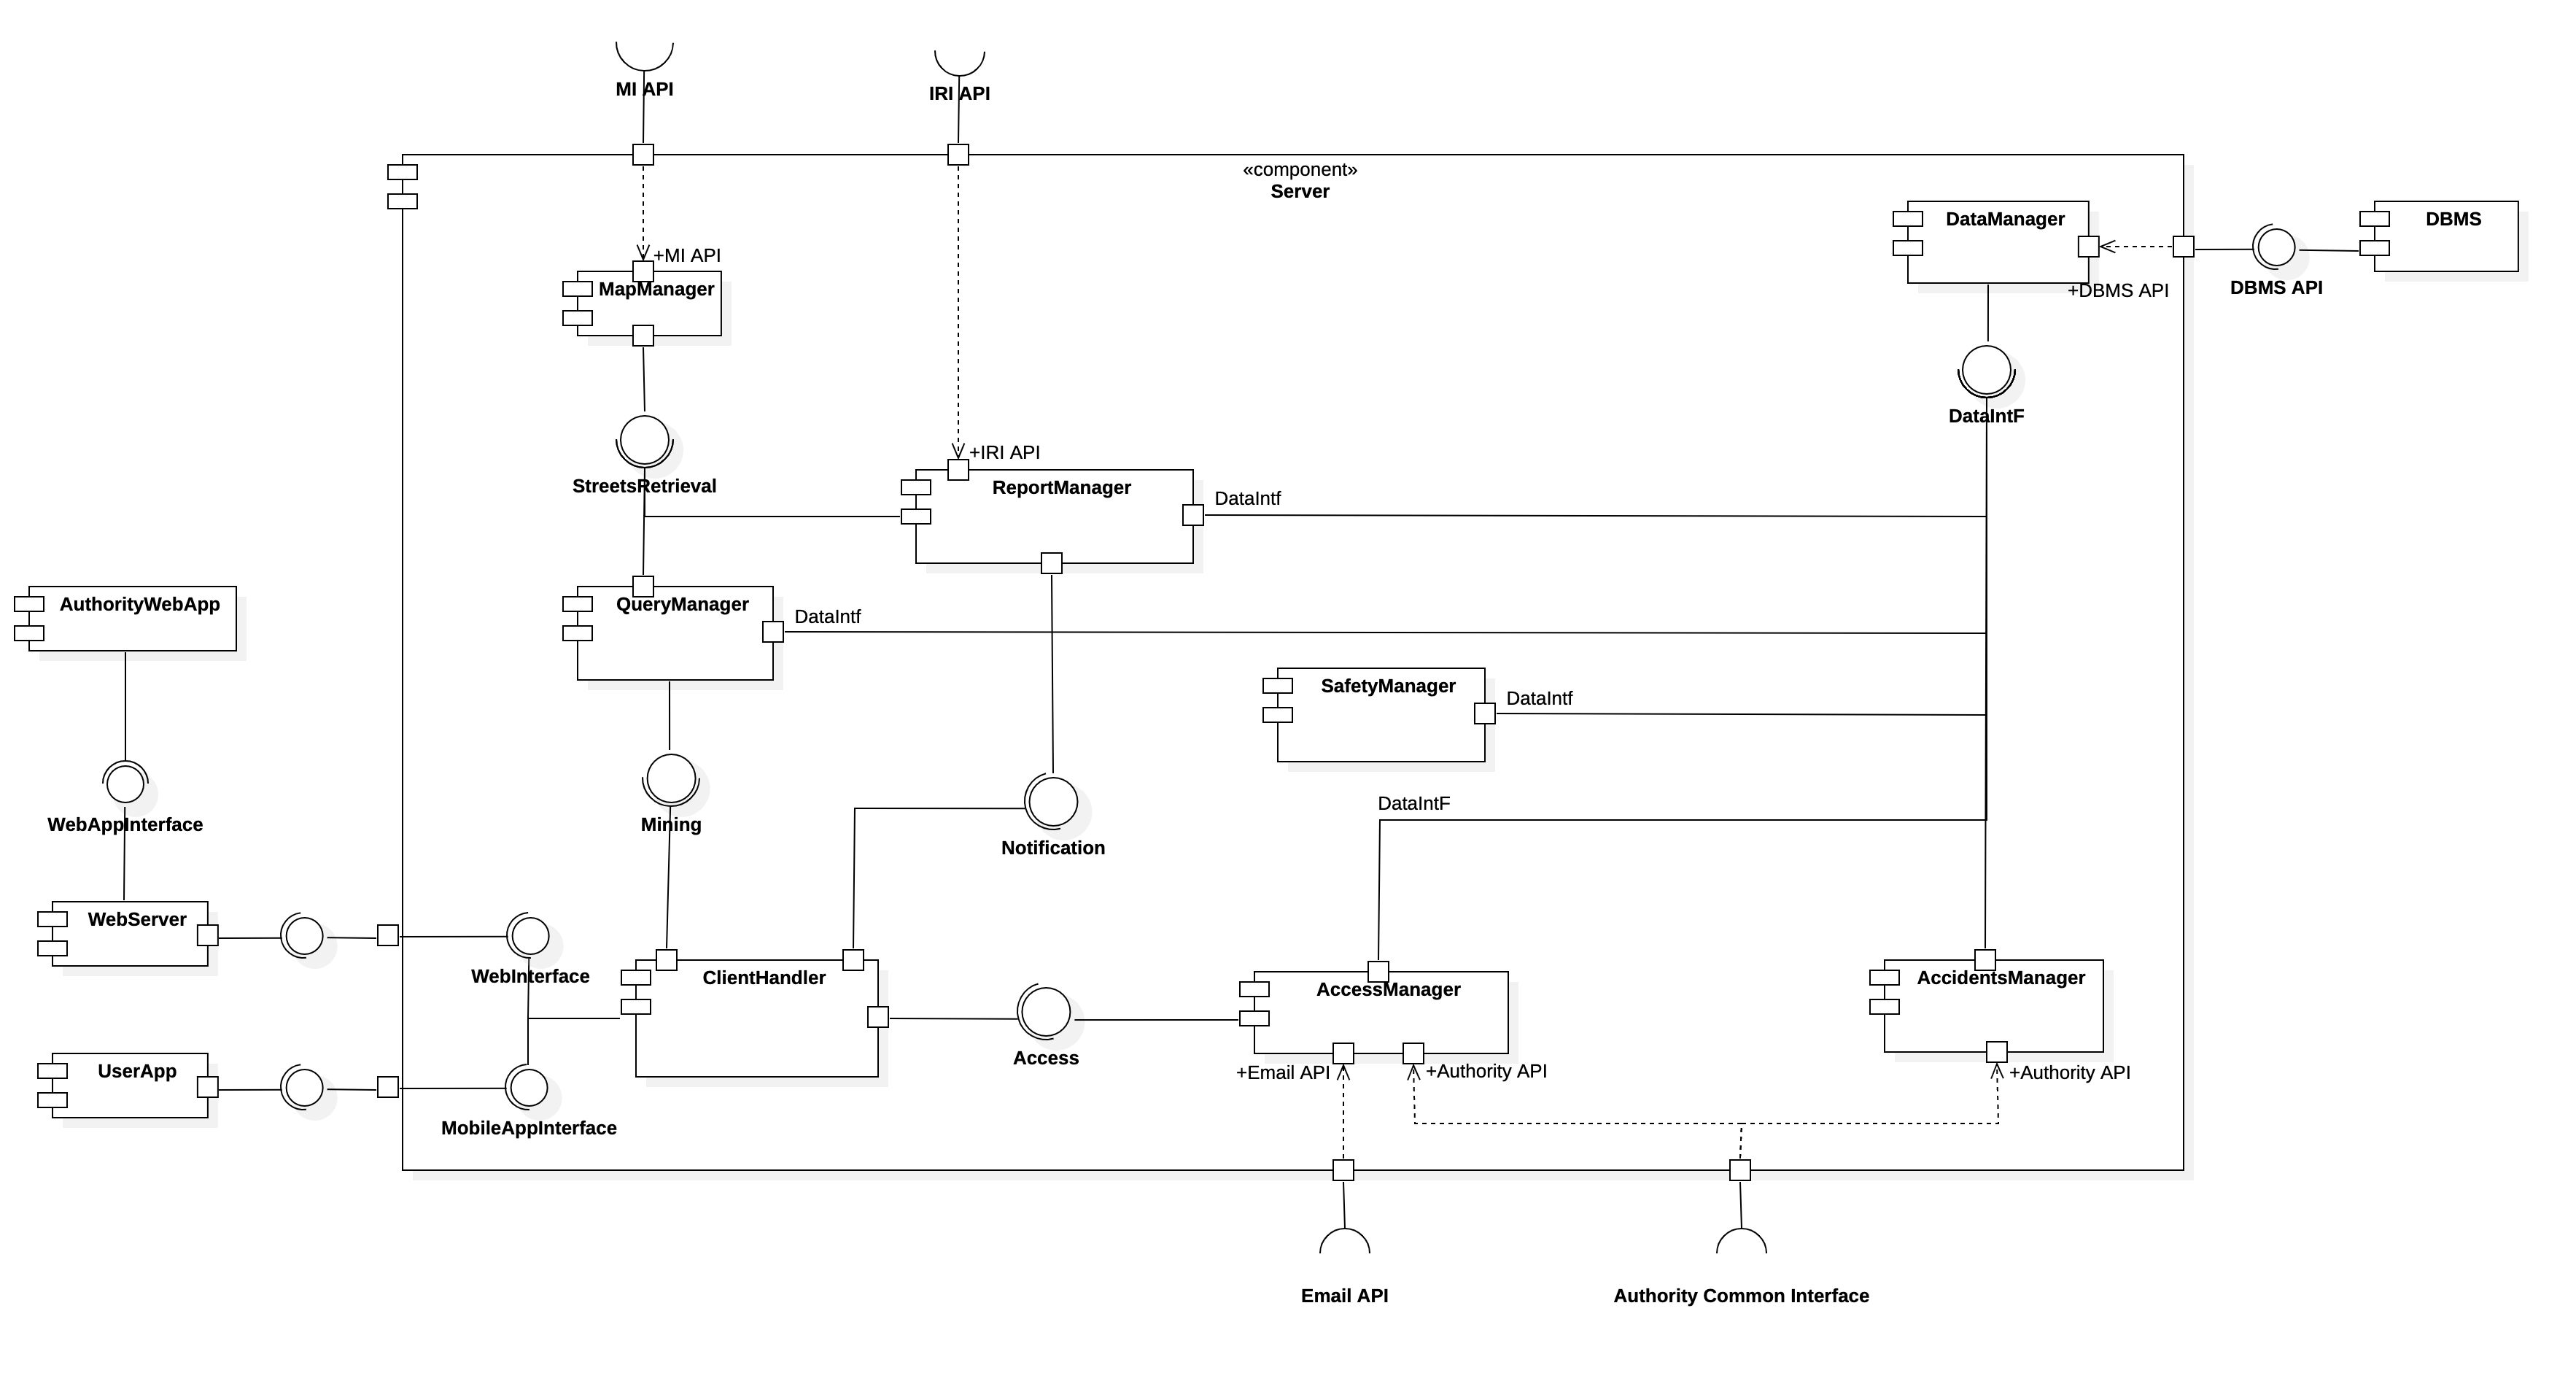
\includegraphics[scale=0.16, angle=90]{/diagrams/components/server.png}
				\caption{\label{fig:serverComp} Server Component Diagram}
			\end{figure}
		
		\subsubsection[Client Handler Component]{\hyperlink{toc}{Client Handler Component}}
			\label{sec:clientHandlerComponent}
			
			\begin{figure}[ht]
				\centering
				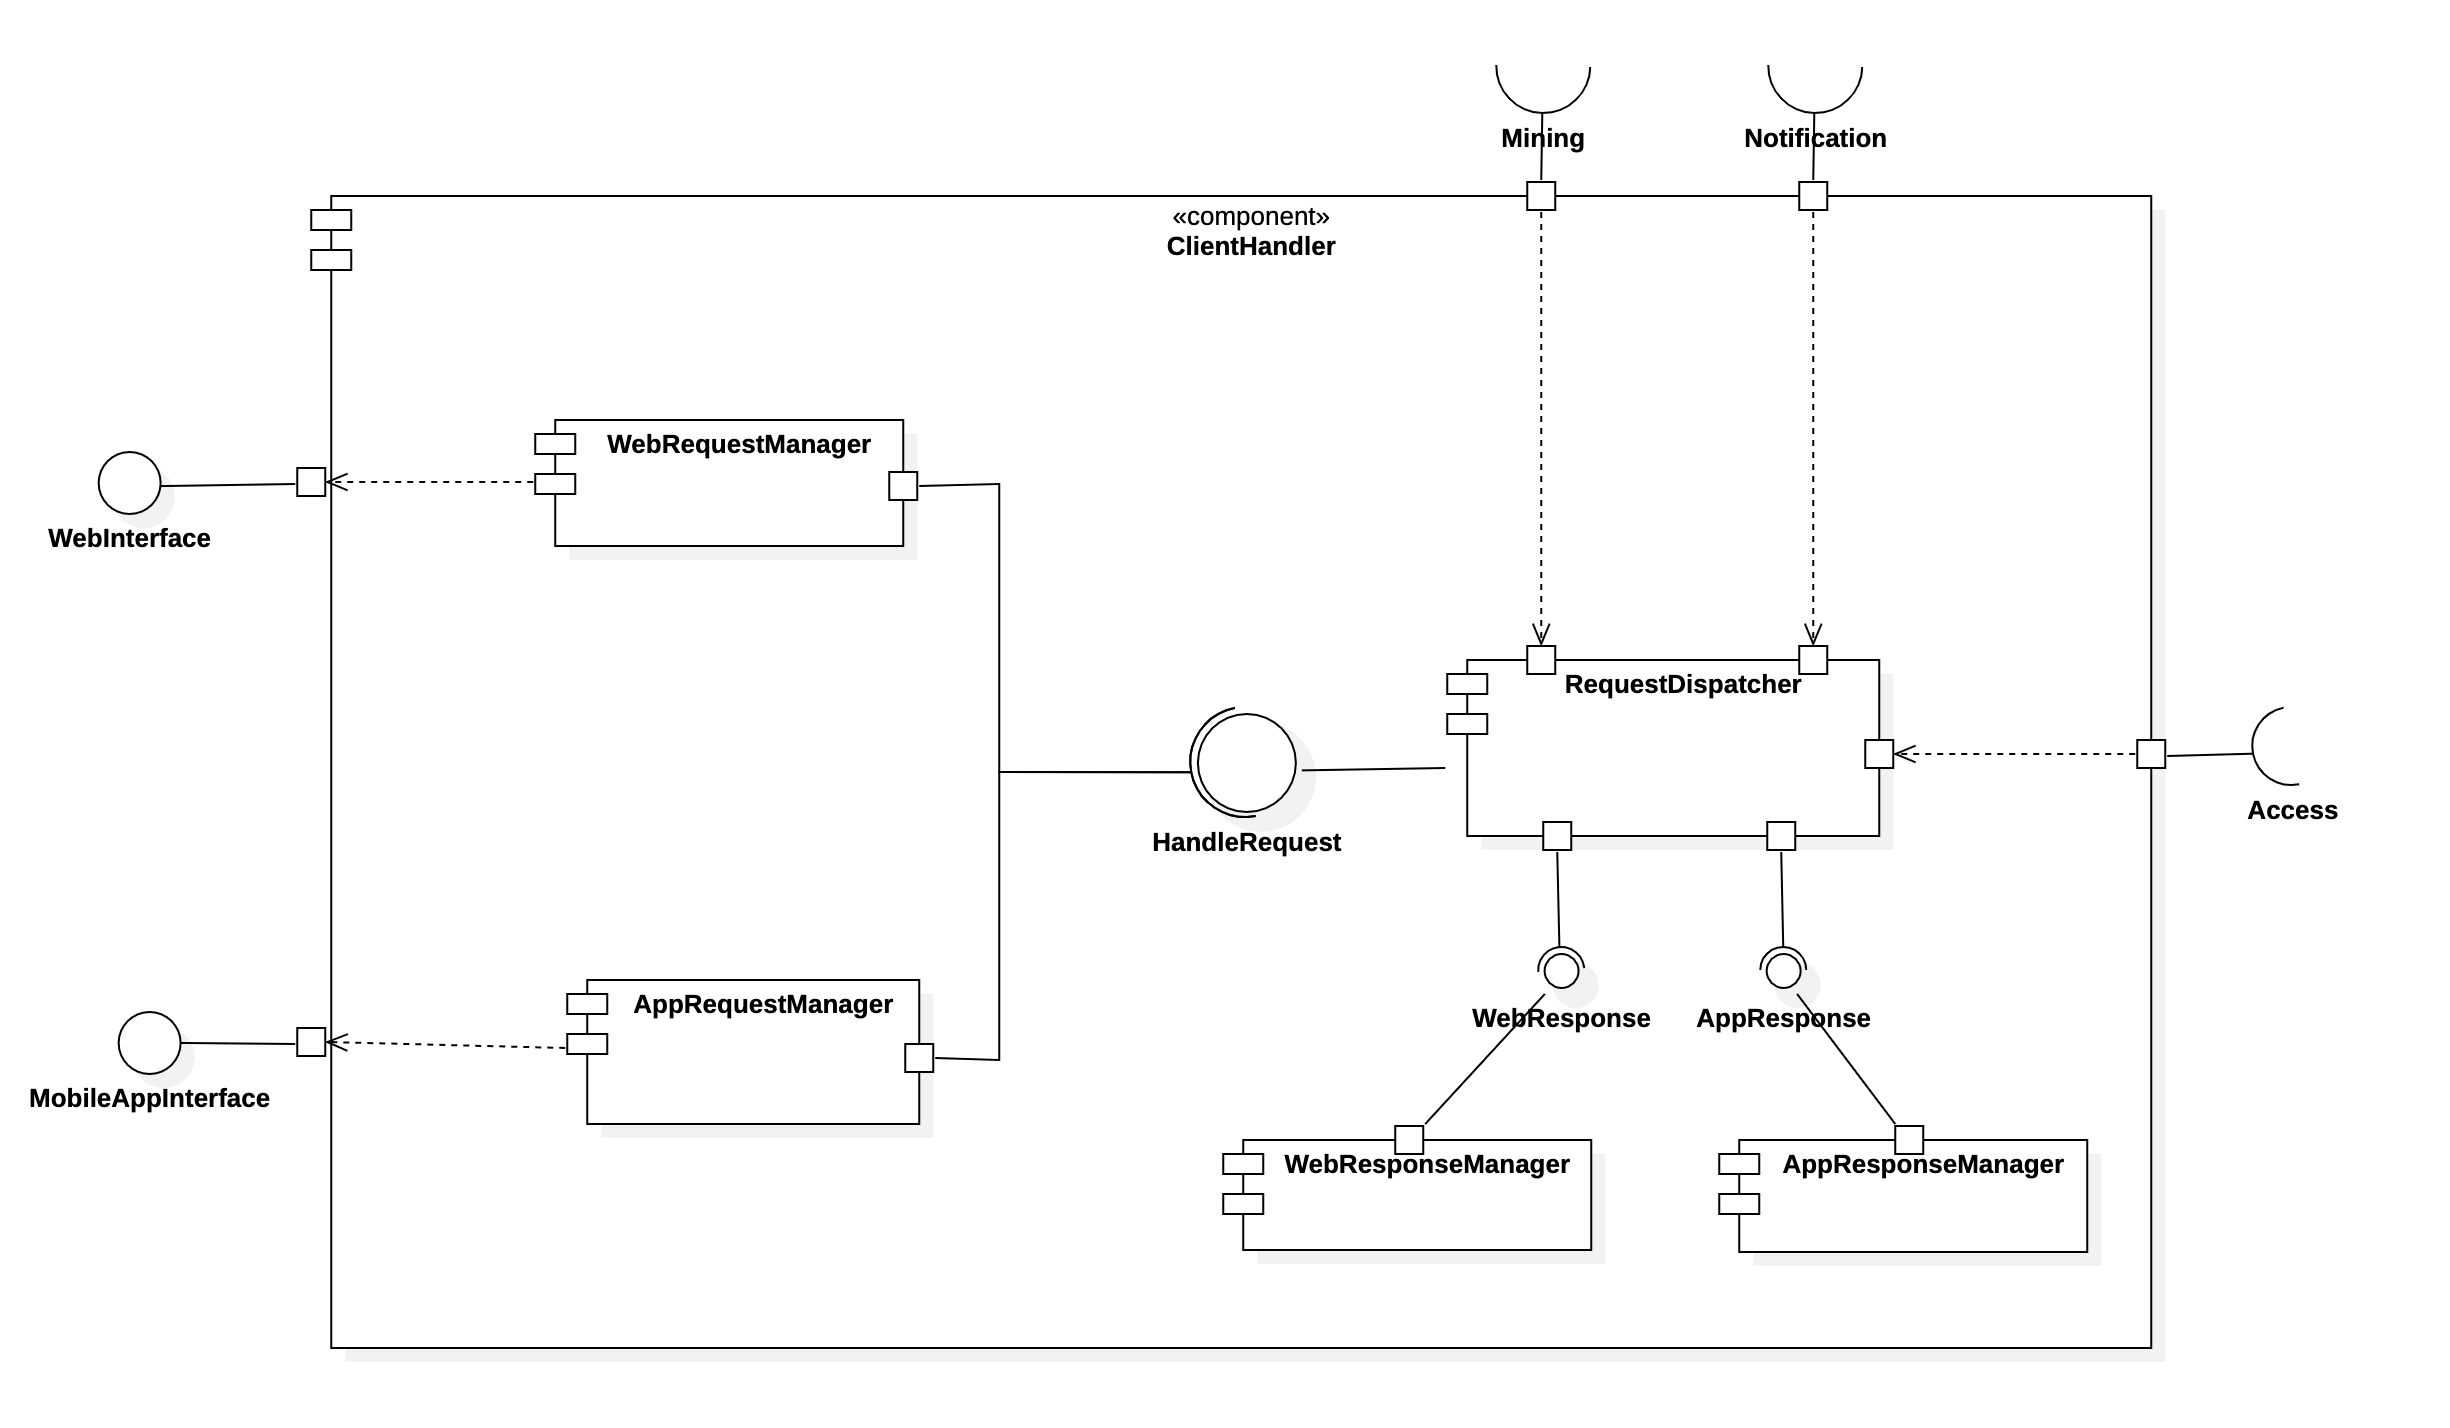
\includegraphics[scale=0.2]{/diagrams/components/clientHandler.png}
				\caption{\label{fig:clientHandlerComp} Client Handler Component Diagram}
			\end{figure}
		
		\subsubsection[Access Manager Component]{\hyperlink{toc}{Access Manager Component}}
			\label{sec:accessManagerComponent}
			
			\begin{figure}[ht]
				\centering
				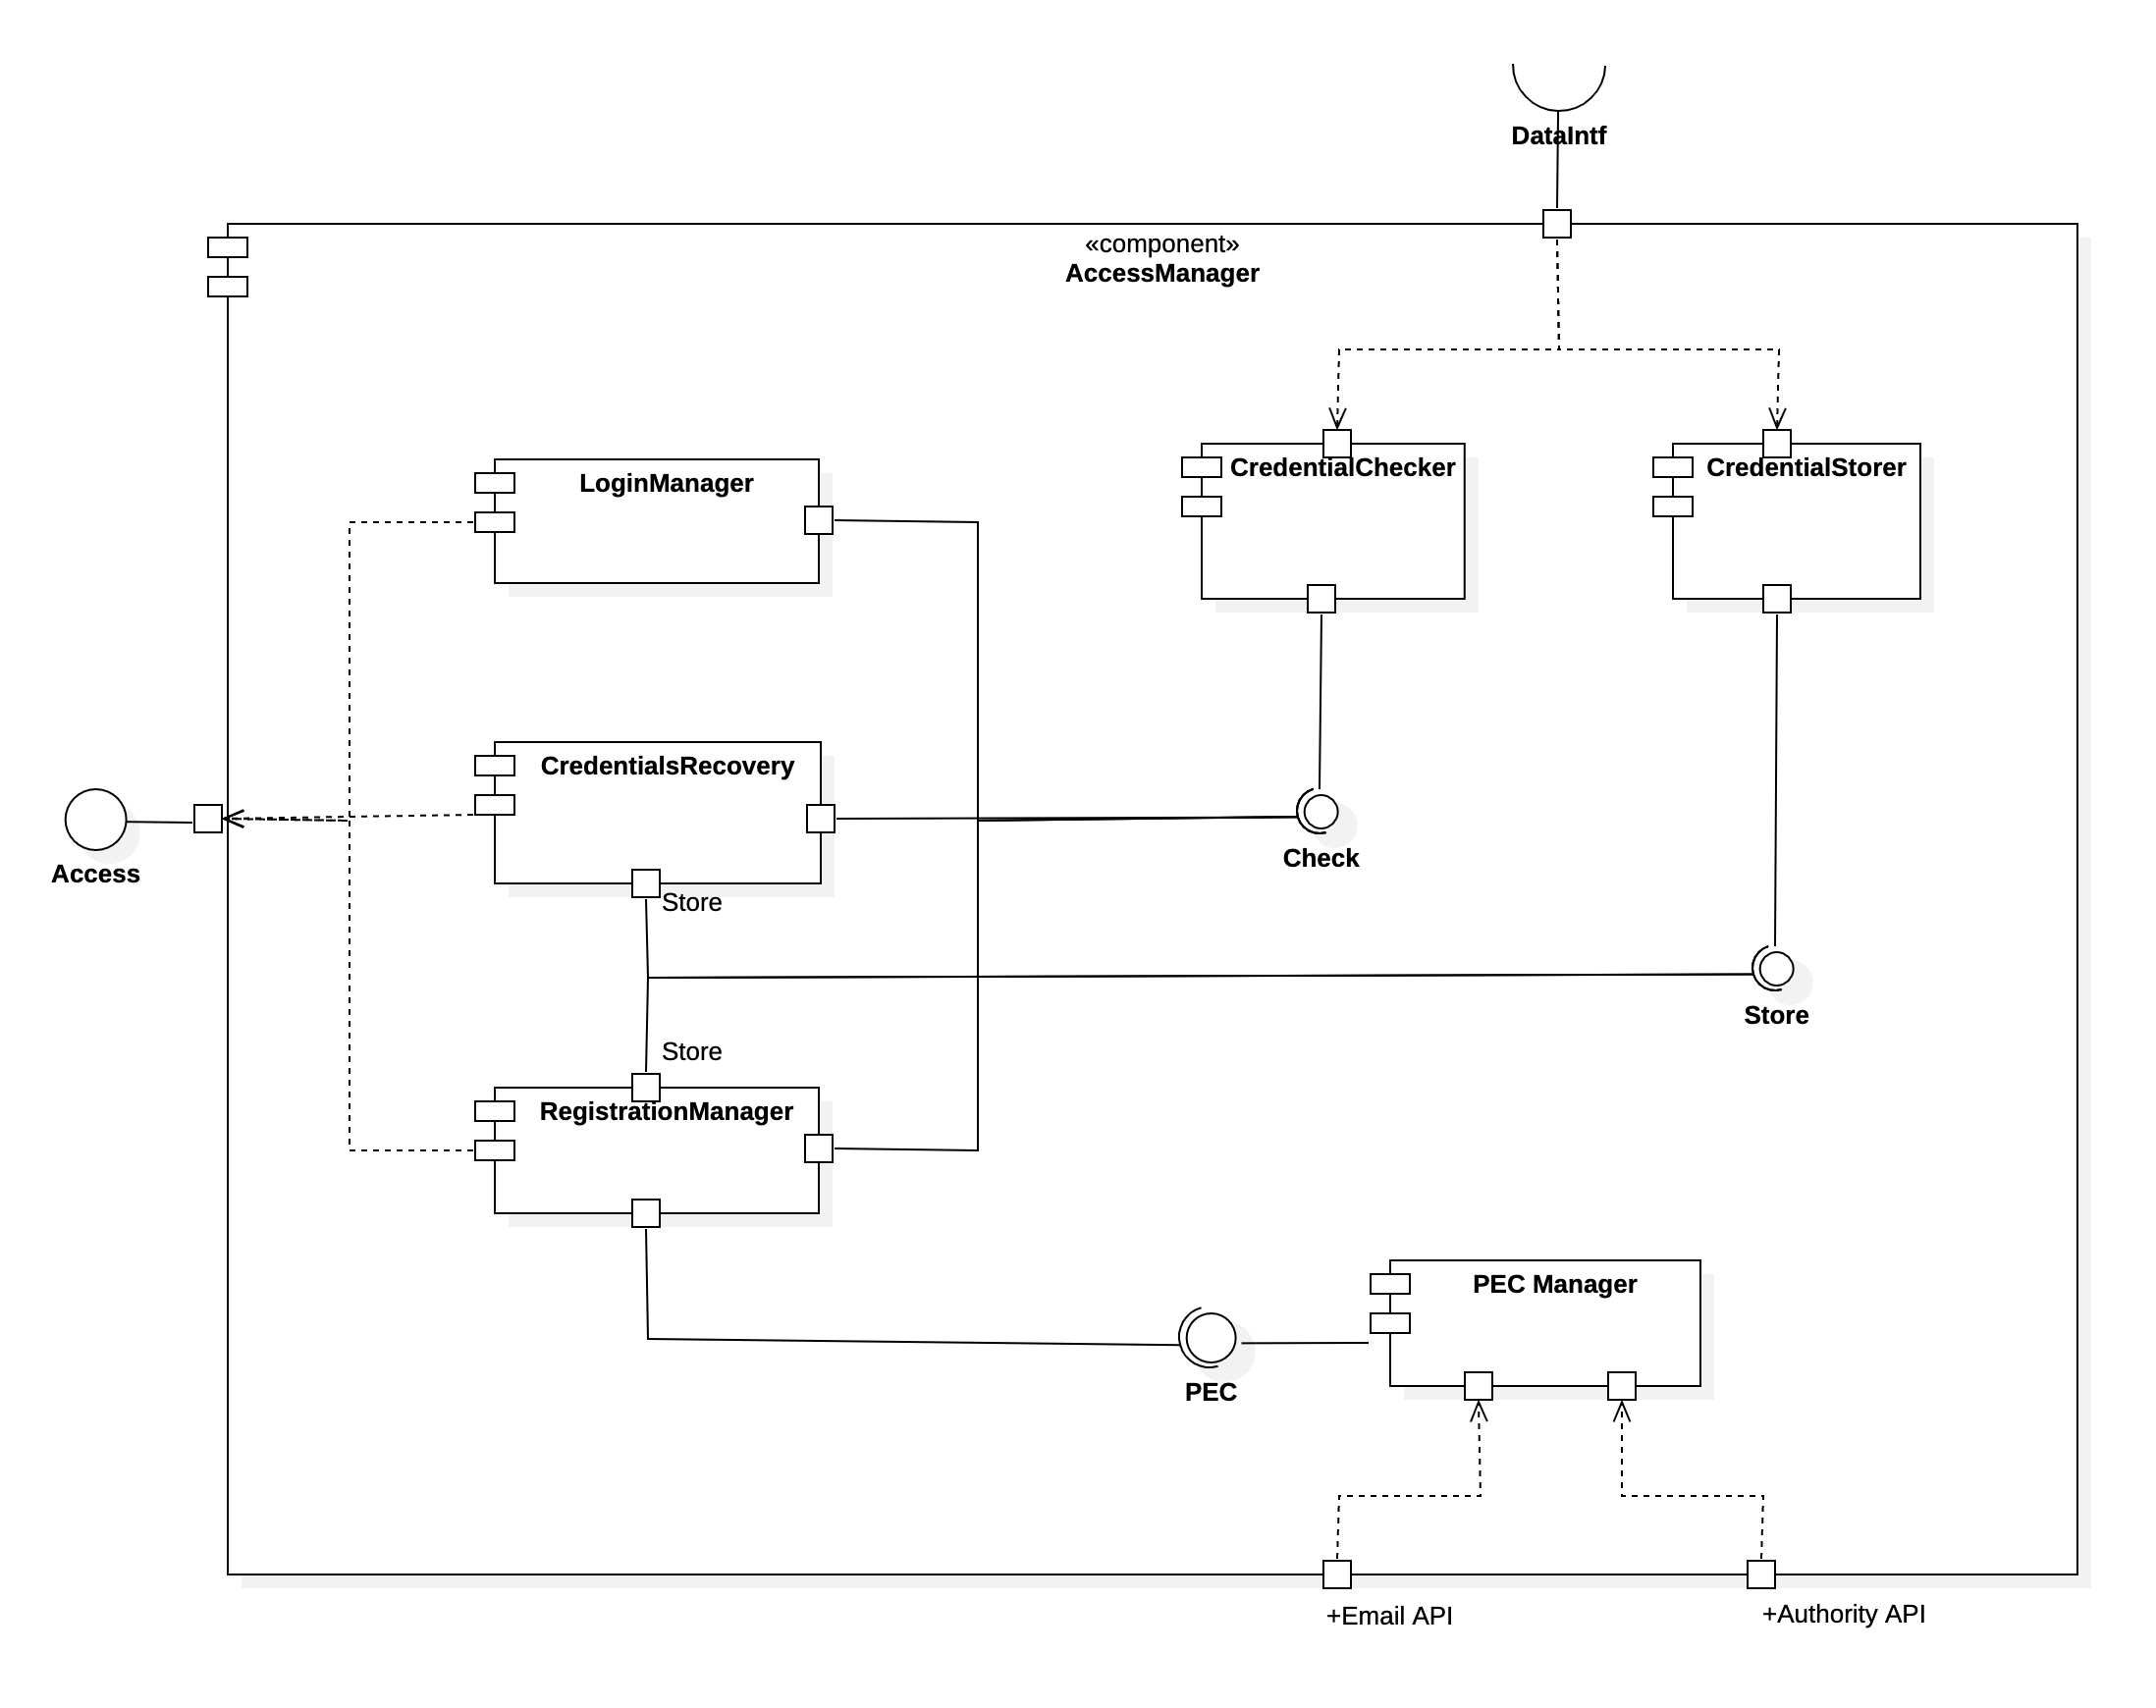
\includegraphics[scale=0.2]{/diagrams/components/accessManager}
				\caption{\label{fig:accessManagerComp} Access Manager Component Diagram}
			\end{figure}
		
		\subsubsection[Query Manager Component]{\hyperlink{toc}{Query Manager Component}}
			\label{sec:queryManagerComponent}
			
			\begin{figure}[ht]
				\centering
				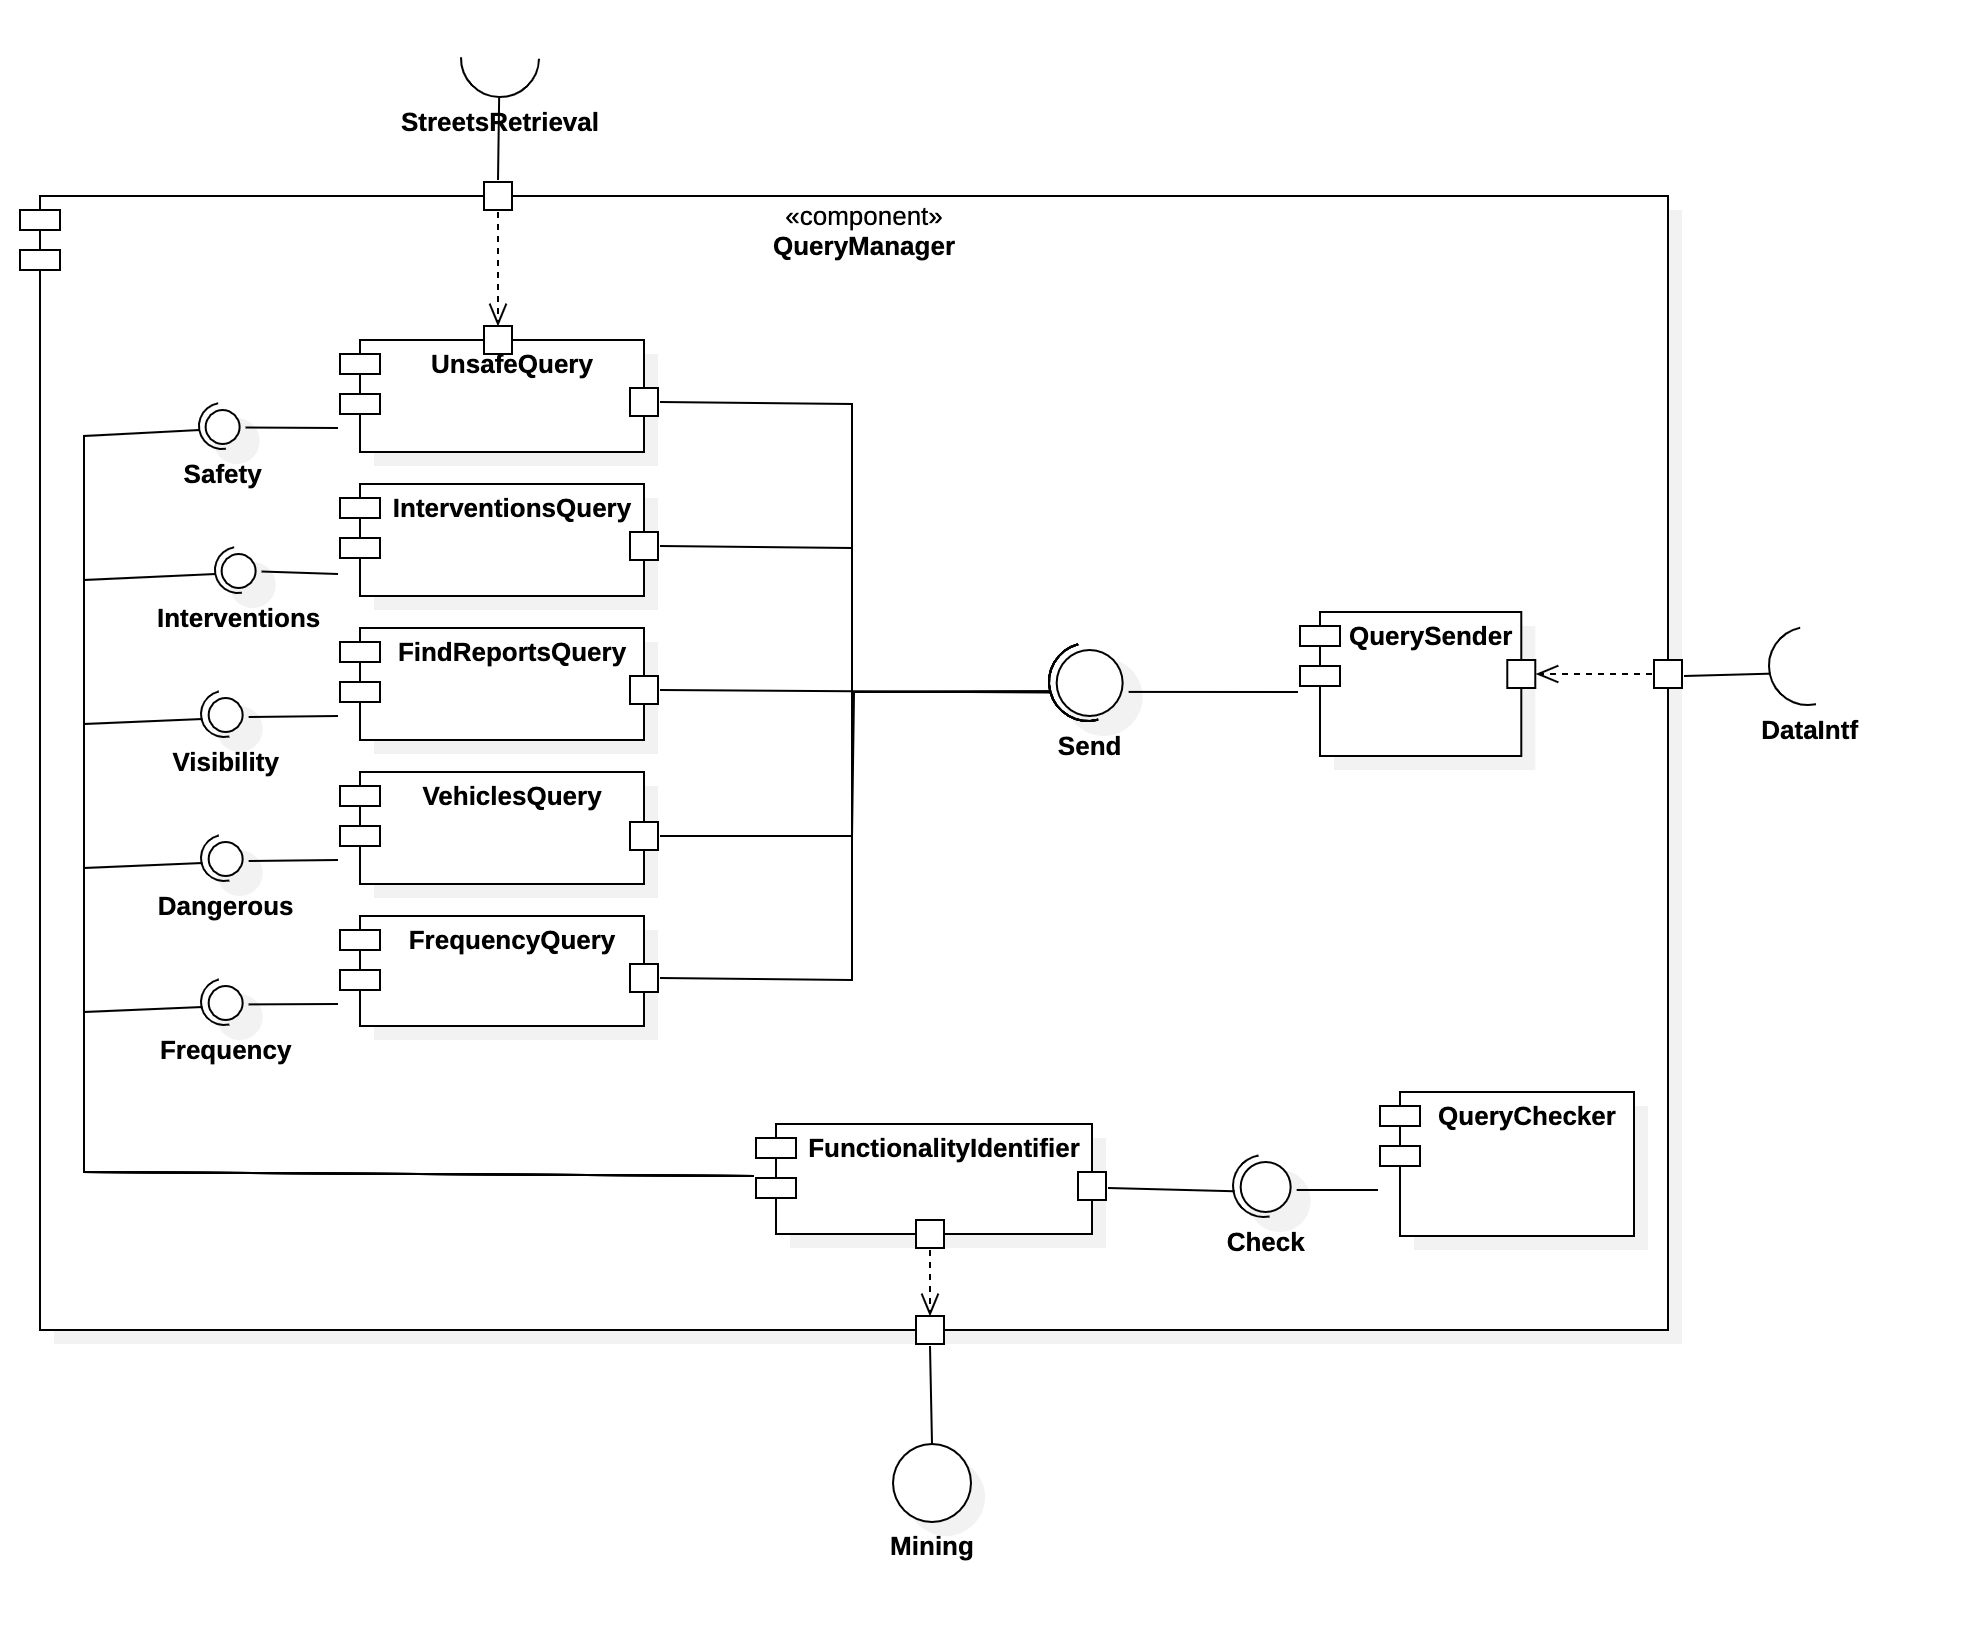
\includegraphics[scale=0.2]{/diagrams/components/queryManager.png}
				\caption{\label{fig:queryManagerComp} Query Manager Component Diagram}
			\end{figure}
		
		\subsubsection[Report Manager Component]{\hyperlink{toc}{Report Manager Component}}
			\label{sec:reportManagerComponent}
			
			\begin{figure}[ht]
				\centering
				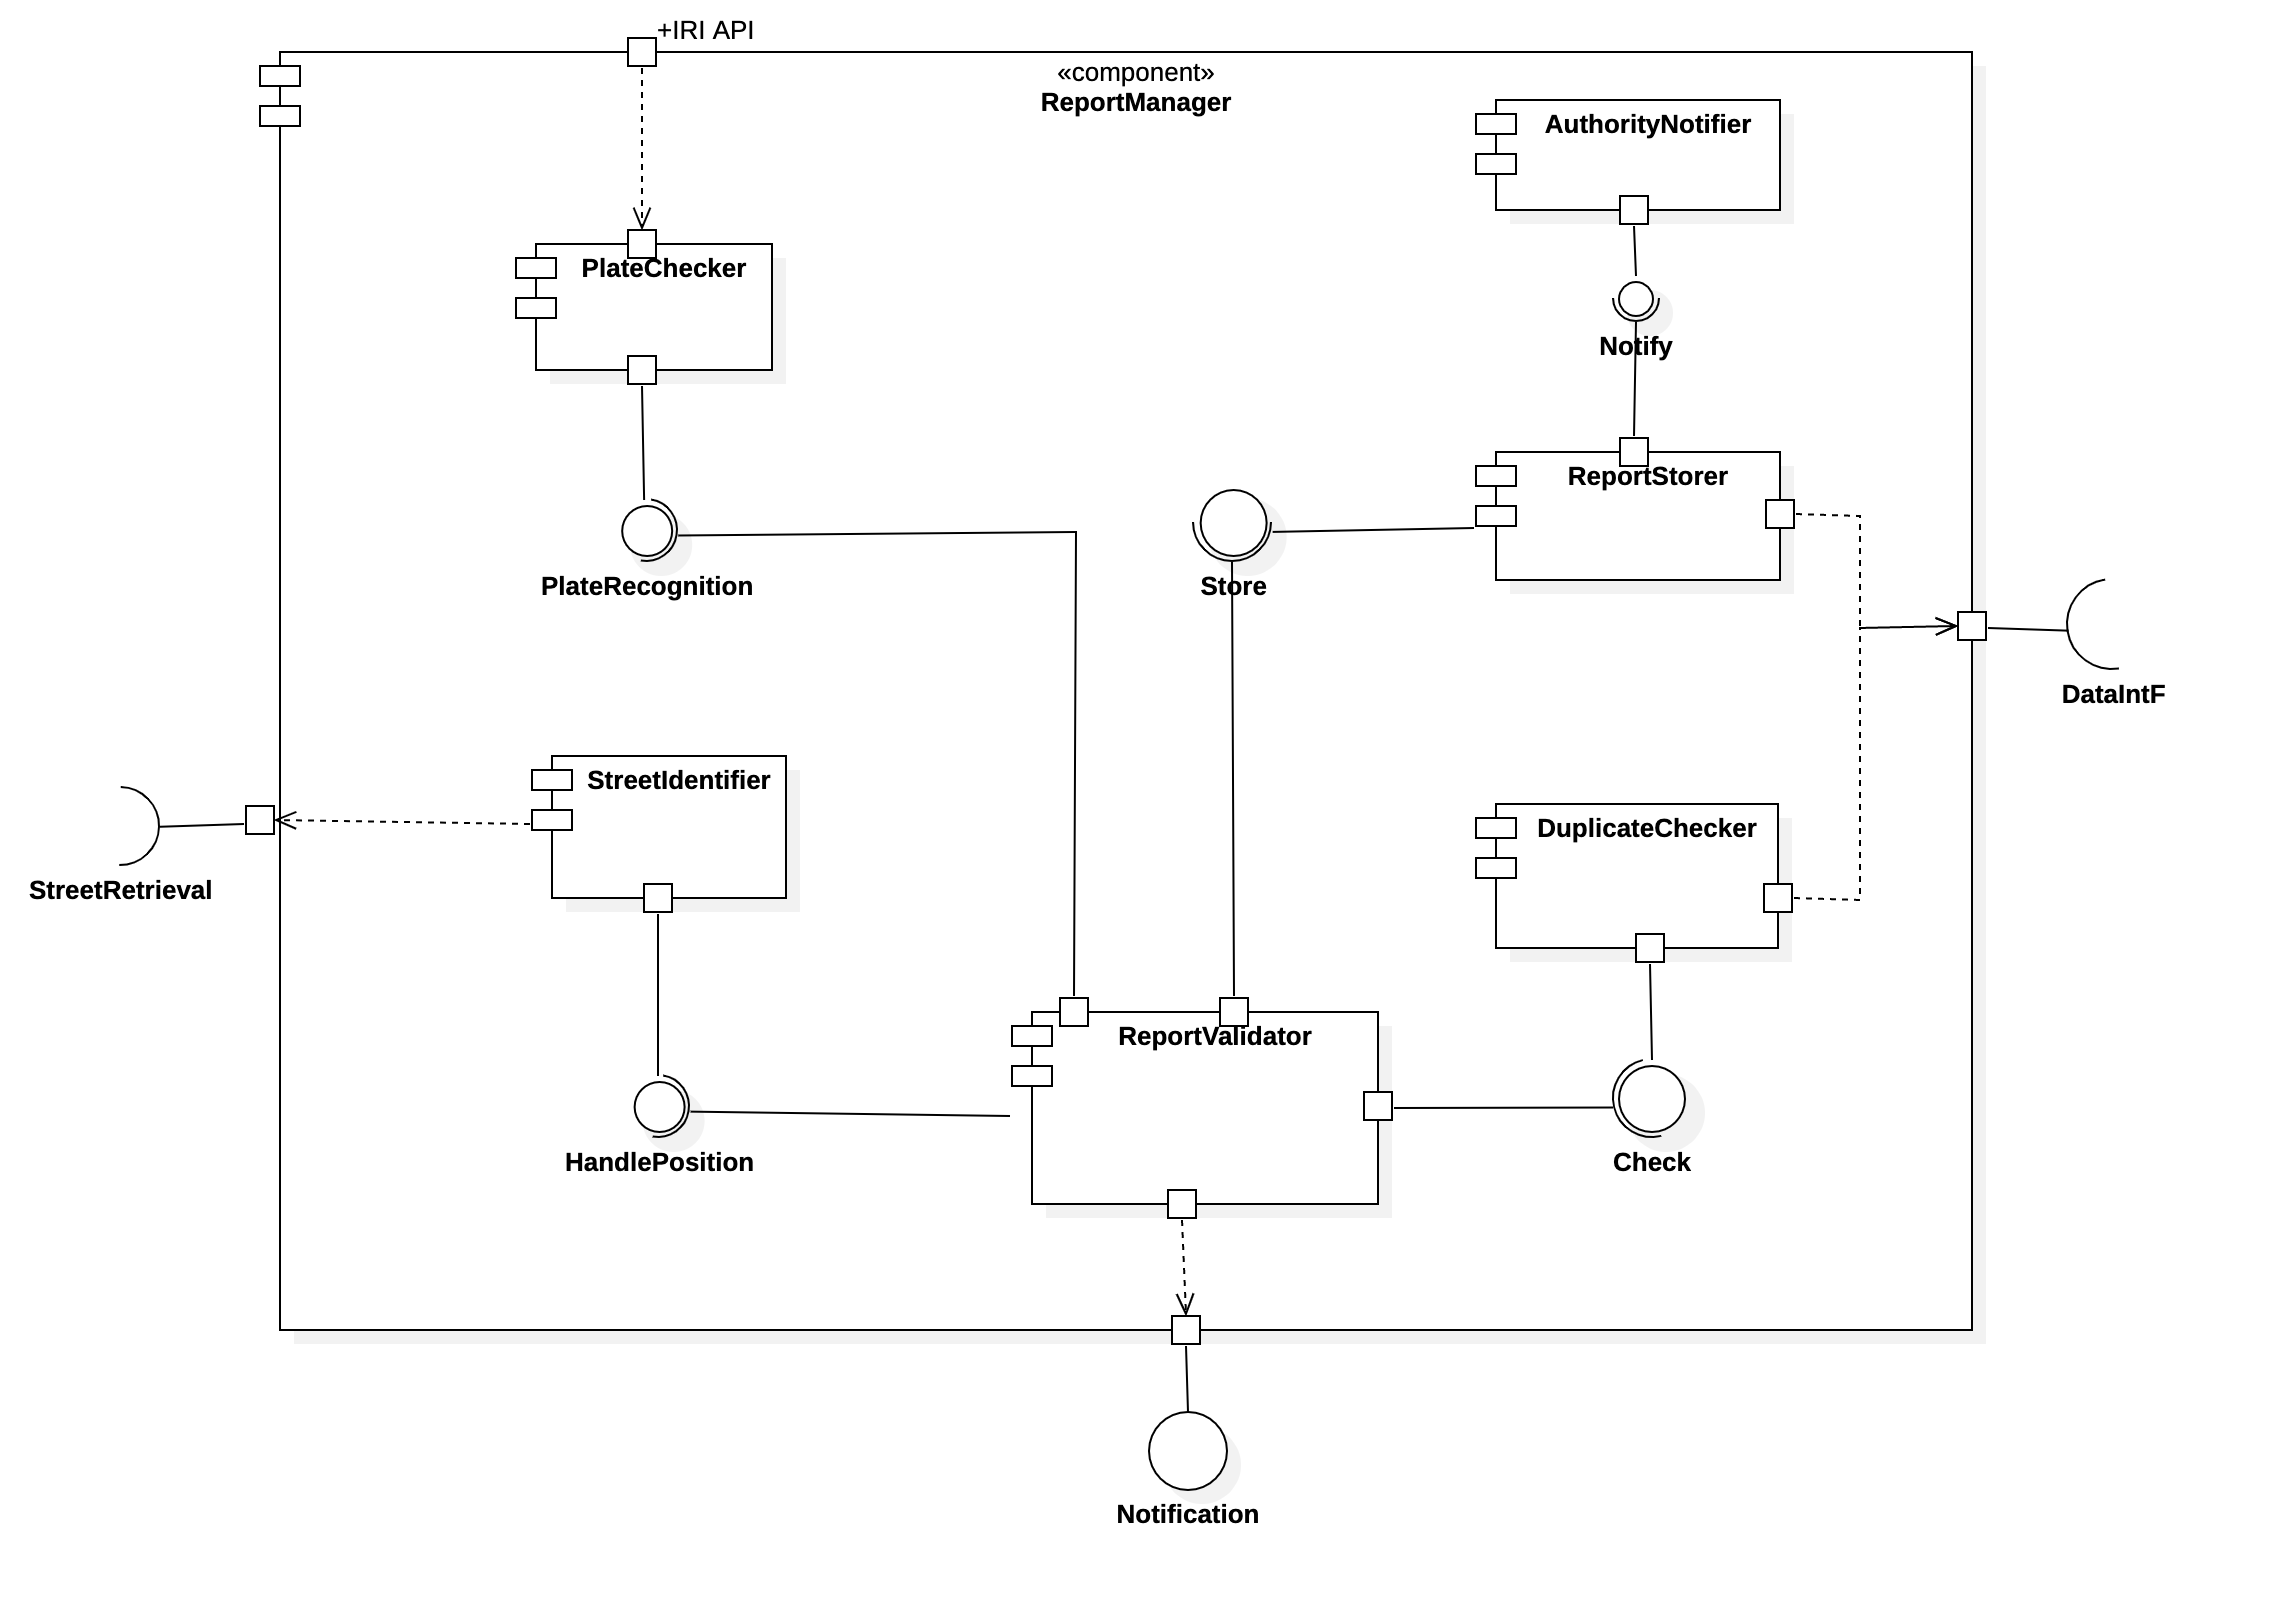
\includegraphics[scale=0.2]{/diagrams/components/reportManager.png}
				\caption{\label{fig:reportManagerComp} Report Manager Component Diagram}
			\end{figure}
		
		\subsubsection[Map Manager Component]{\hyperlink{toc}{Map Manager Component}}
			\label{sec:mapManagerComponent}
			
			\begin{figure}[ht]
				\centering
				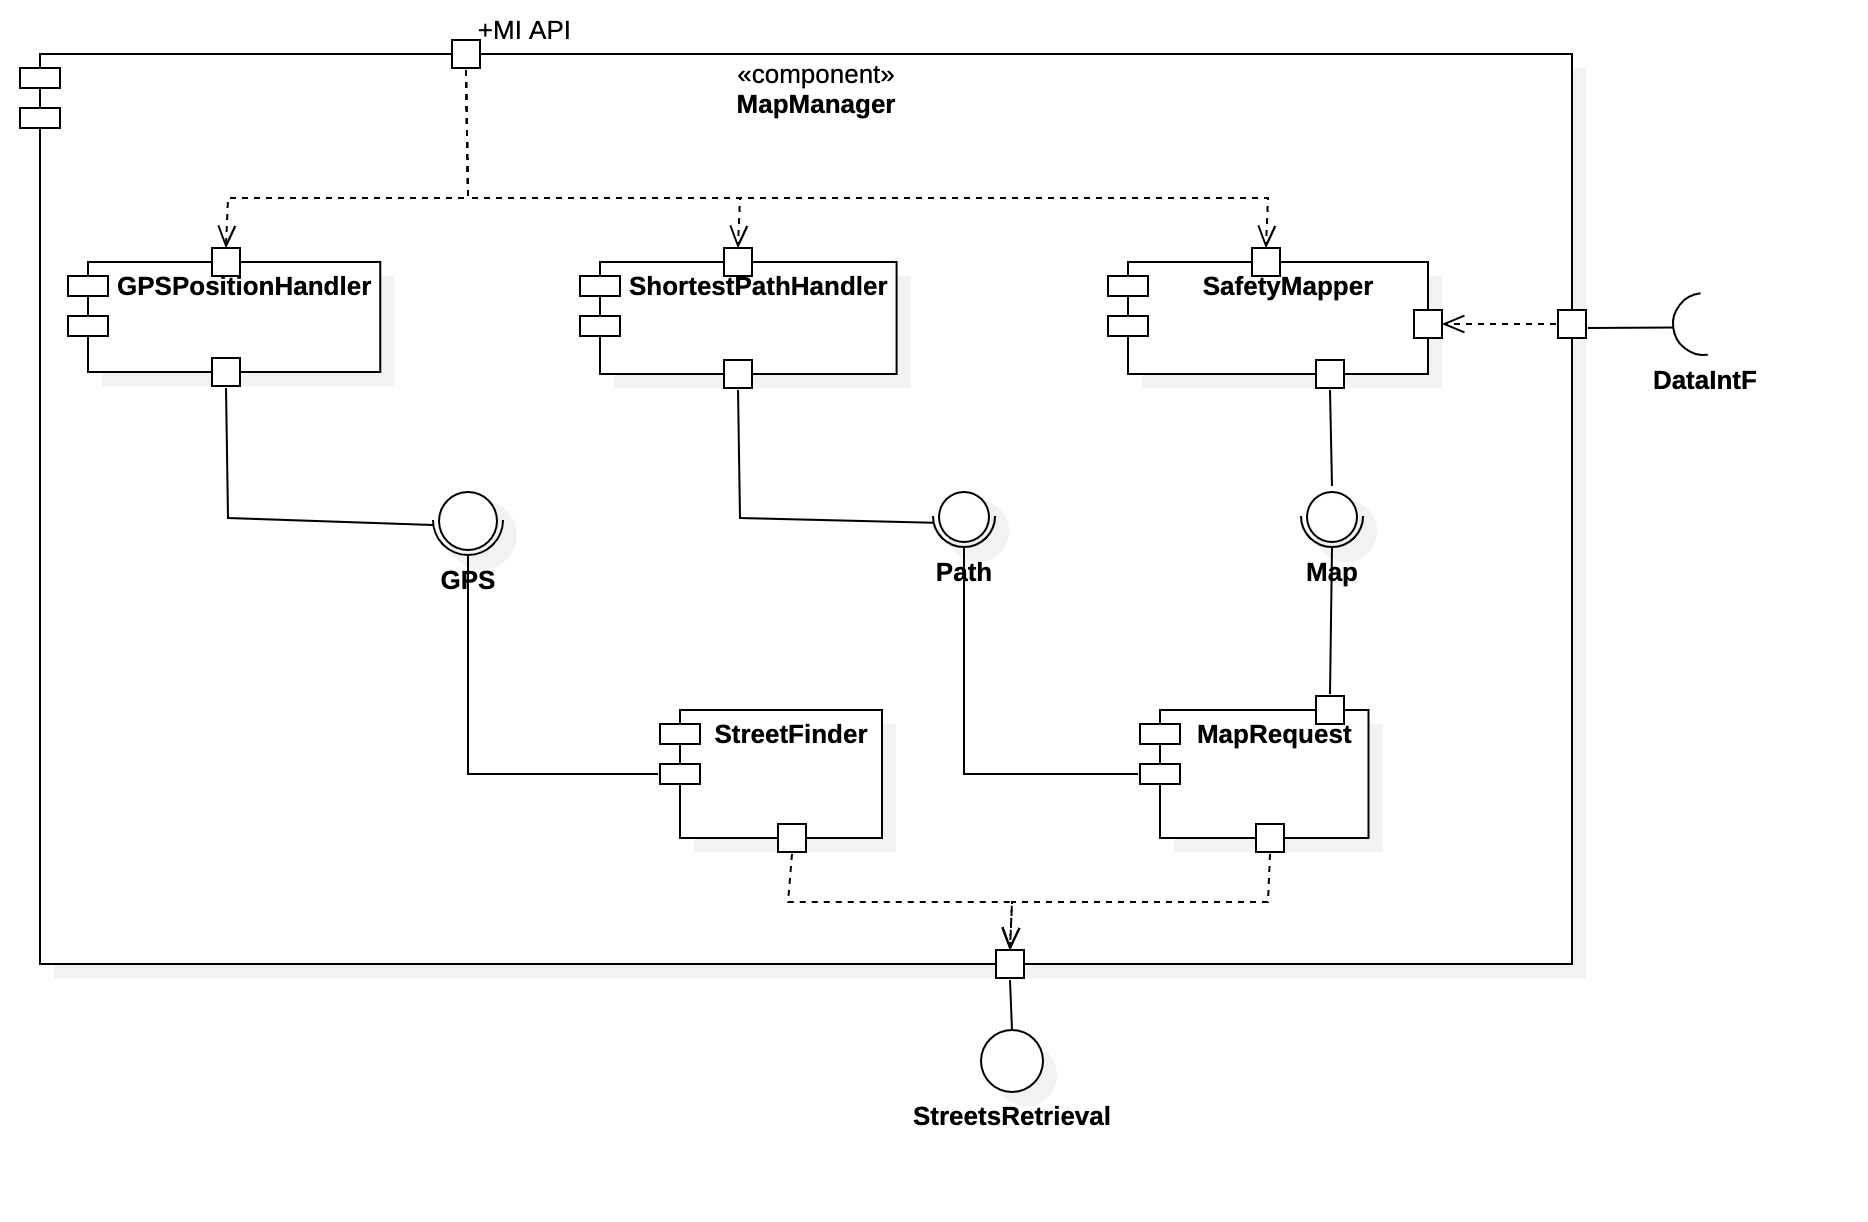
\includegraphics[scale=0.2]{/diagrams/components/mapManager.png}
				\caption{\label{fig:mapManagerComp} Map Manager Component Diagram}
			\end{figure}
		
		\subsubsection[Safety Manager Component]{\hyperlink{toc}{Safety Manager Component}}
			\label{sec:safetyManagerComponent}
			
			\begin{figure}[ht]
				\centering
				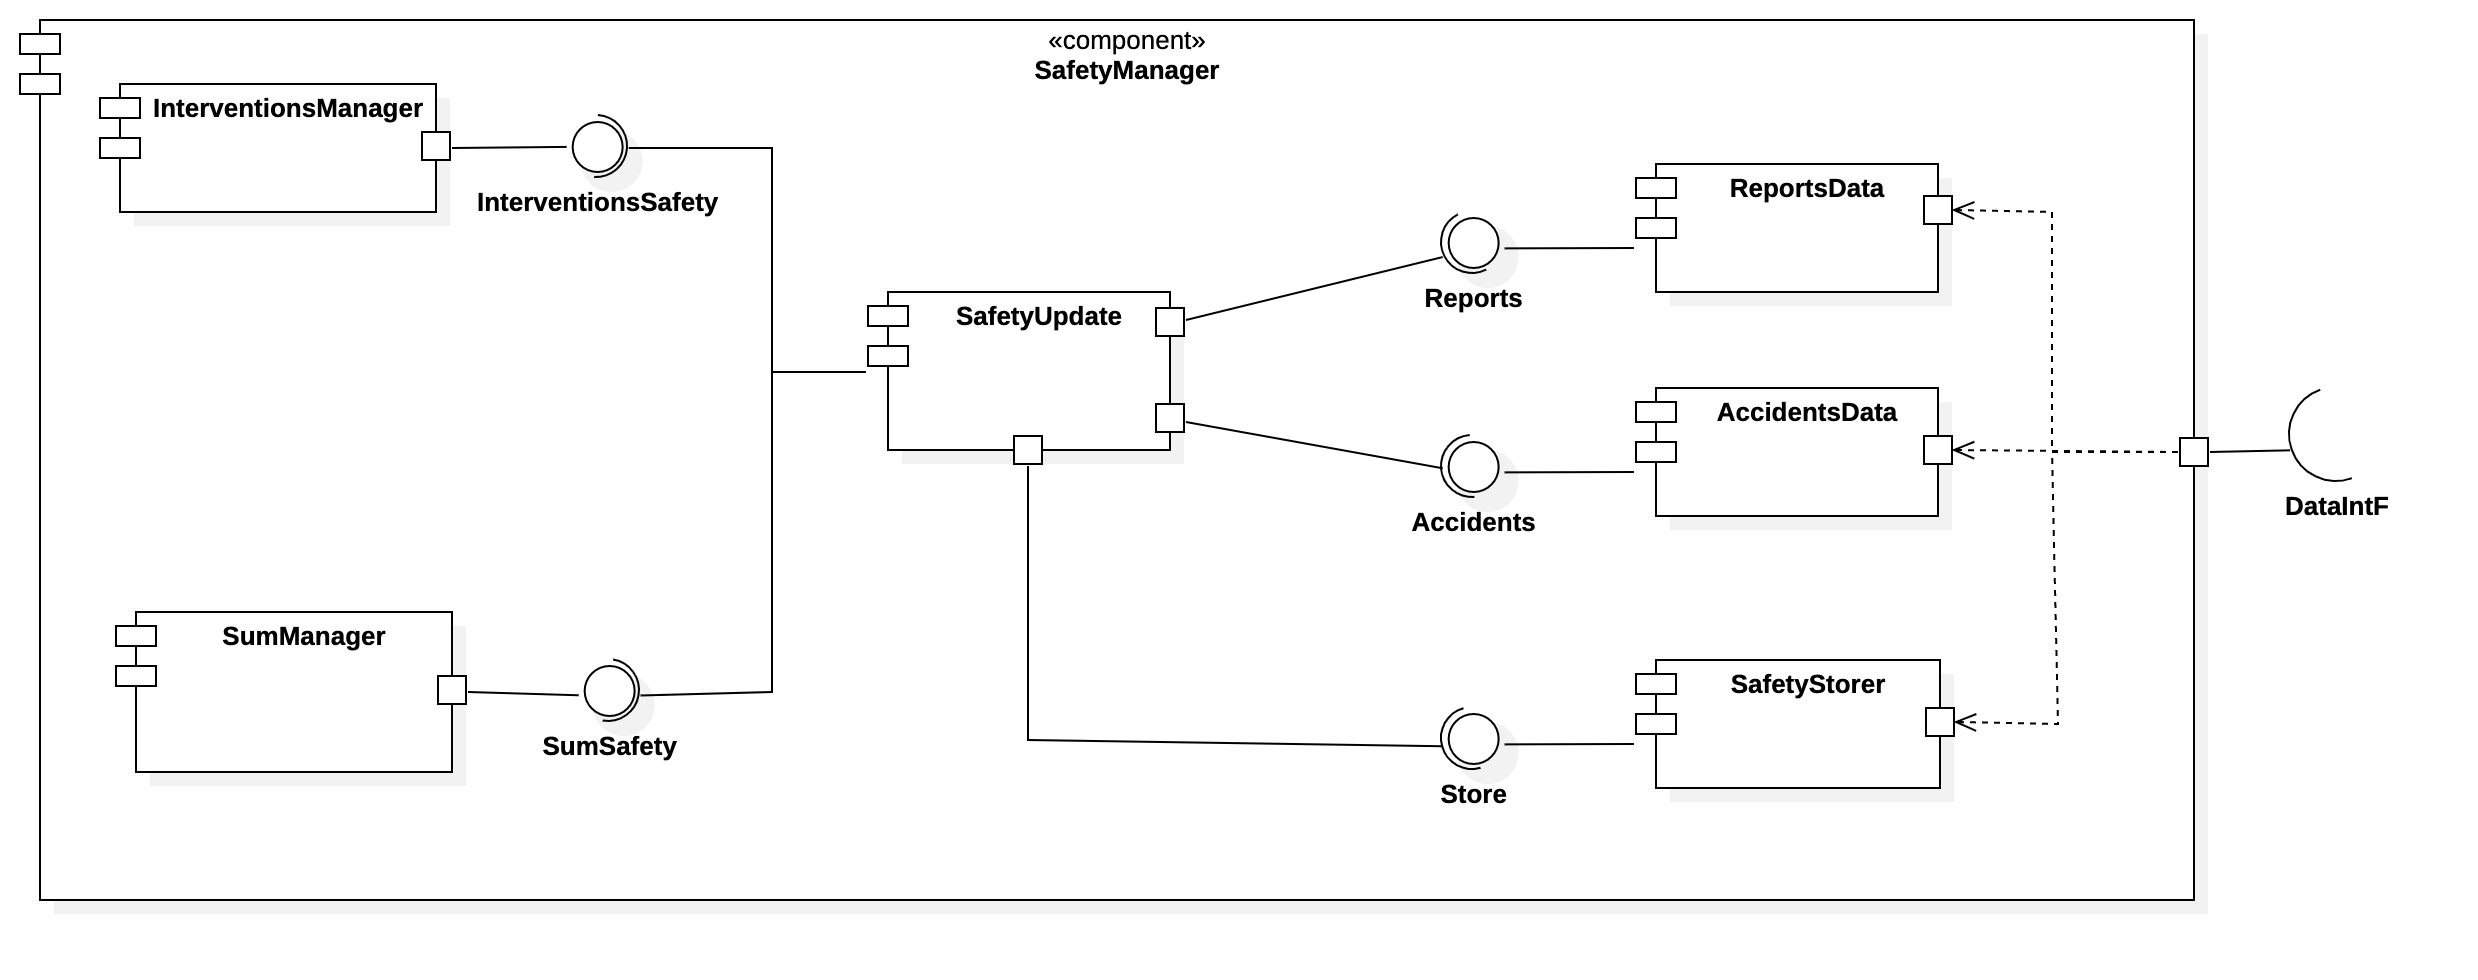
\includegraphics[scale=0.2]{/diagrams/components/safetyManager.png}
				\caption{\label{fig:safetyManagerComp} Safety Manager Component Diagram}
			\end{figure}
		
		\subsubsection[Accidents Manager Component]{\hyperlink{toc}{Accidents Manager Component}}
			\label{sec:accidentsManagerComponent}
			
			\begin{figure}[ht]
				\centering
				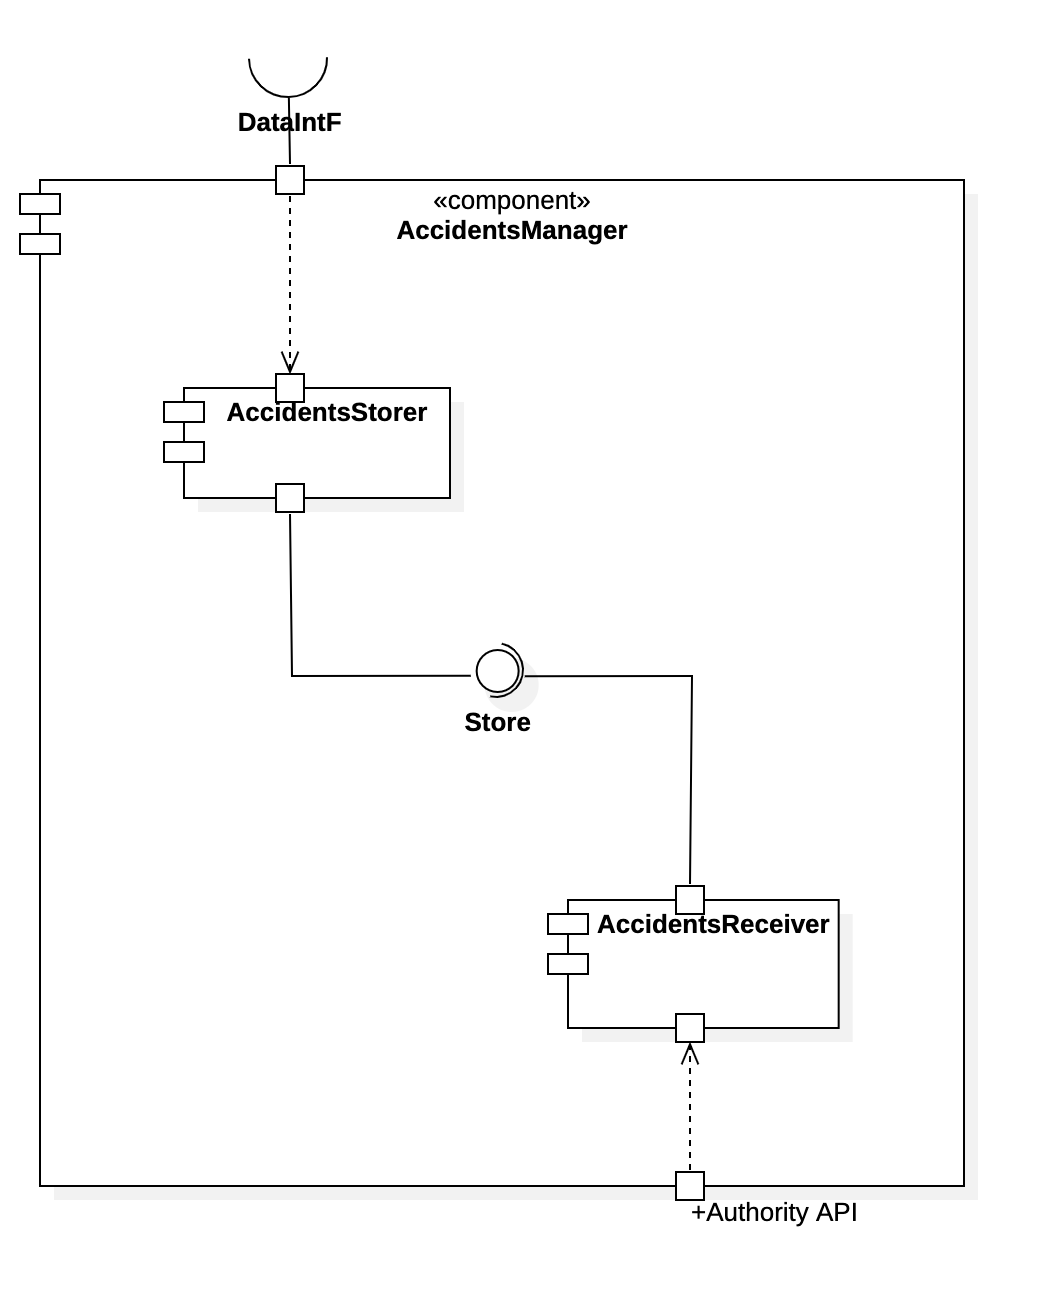
\includegraphics[scale=0.2]{/diagrams/components/accidentsManager.png}
				\caption{\label{fig:accidentsManagerComp} Accidents Manager Component Diagram}
			\end{figure}
		
		\subsubsection[Data Manager Component]{\hyperlink{toc}{Data Manager Component}}
			\label{sec:dataManagerComponent}
			
			\begin{figure}[ht]
				\centering
				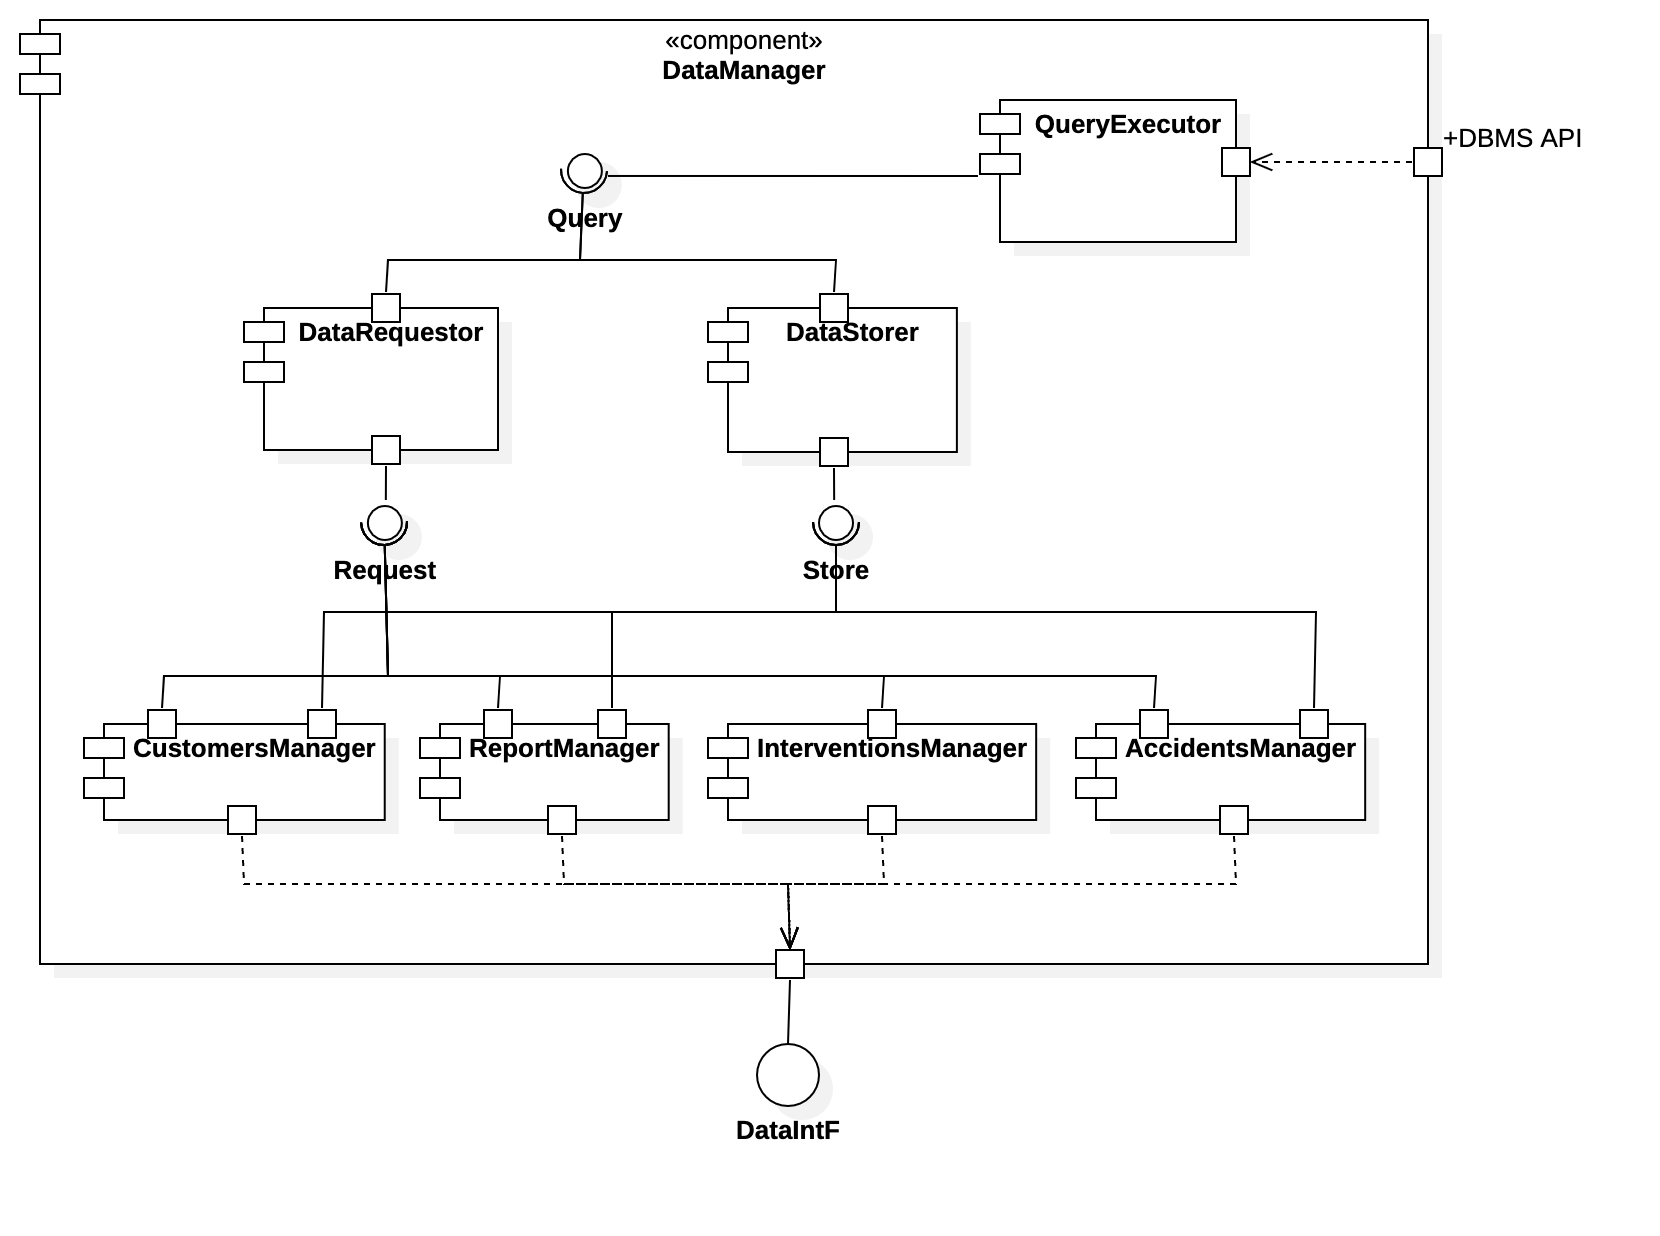
\includegraphics[scale=0.2]{/diagrams/components/dataManager.png}
				\caption{\label{fig:dataManagerComp} Data Manager Component Diagram}
			\end{figure}
		
		\subsubsection[Web Server Component]{\hyperlink{toc}{Web Server Component}}
			\label{sec:webServerComponent}
			
			\begin{figure}[ht]
				\centering
				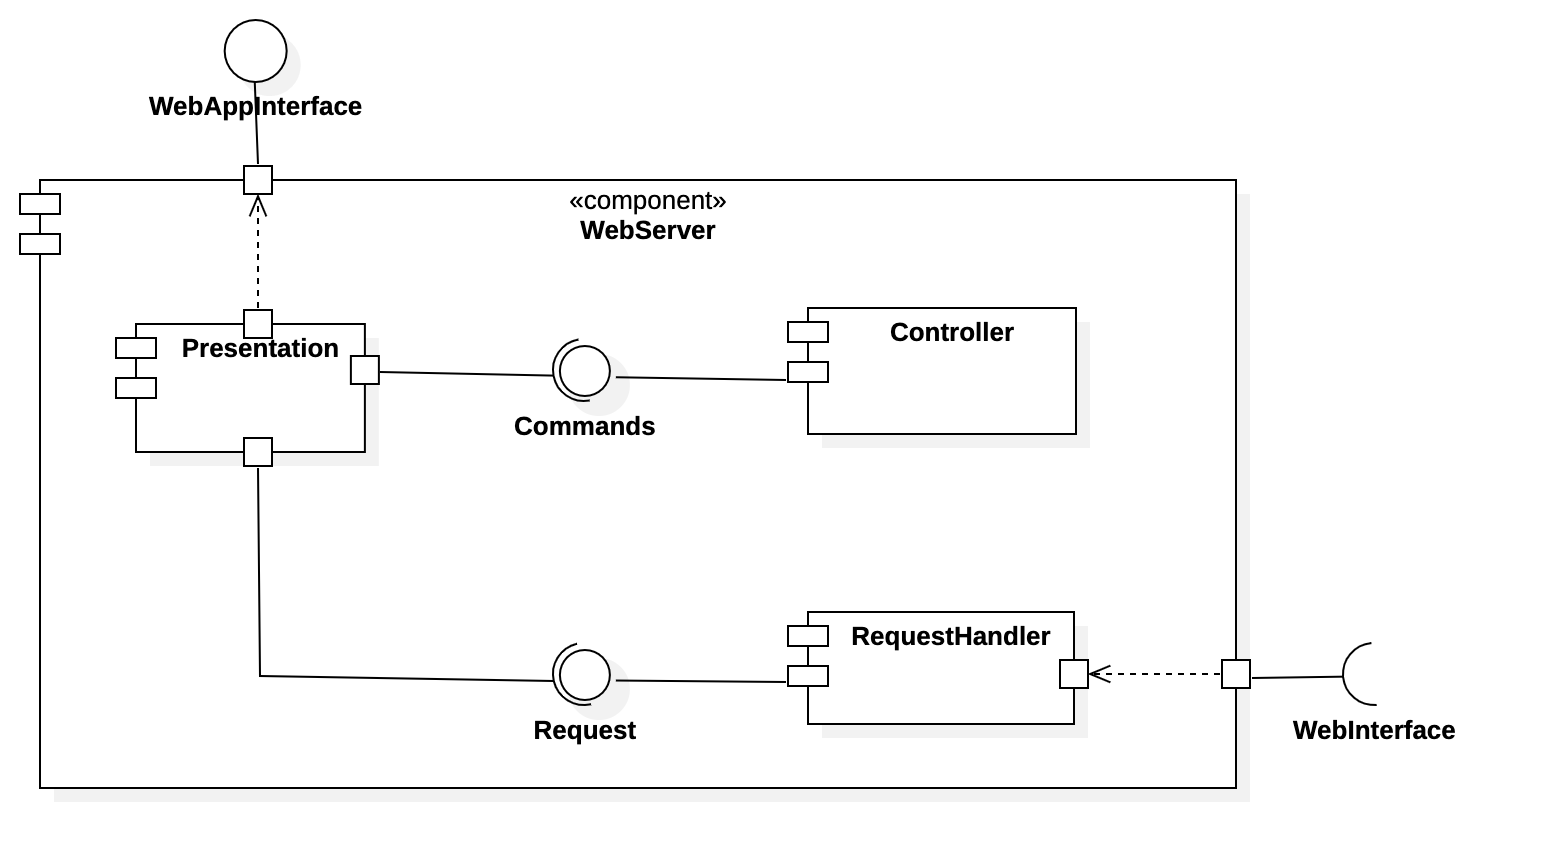
\includegraphics[scale=0.2]{/diagrams/components/webServer.png}
				\caption{\label{fig:webServerComp} Web Server Component Diagram}
			\end{figure}
		
		\subsubsection[User App Component]{\hyperlink{toc}{User App Component}}
			\label{sec:userAppComponent}
			
			\begin{figure}[ht]
				\centering
				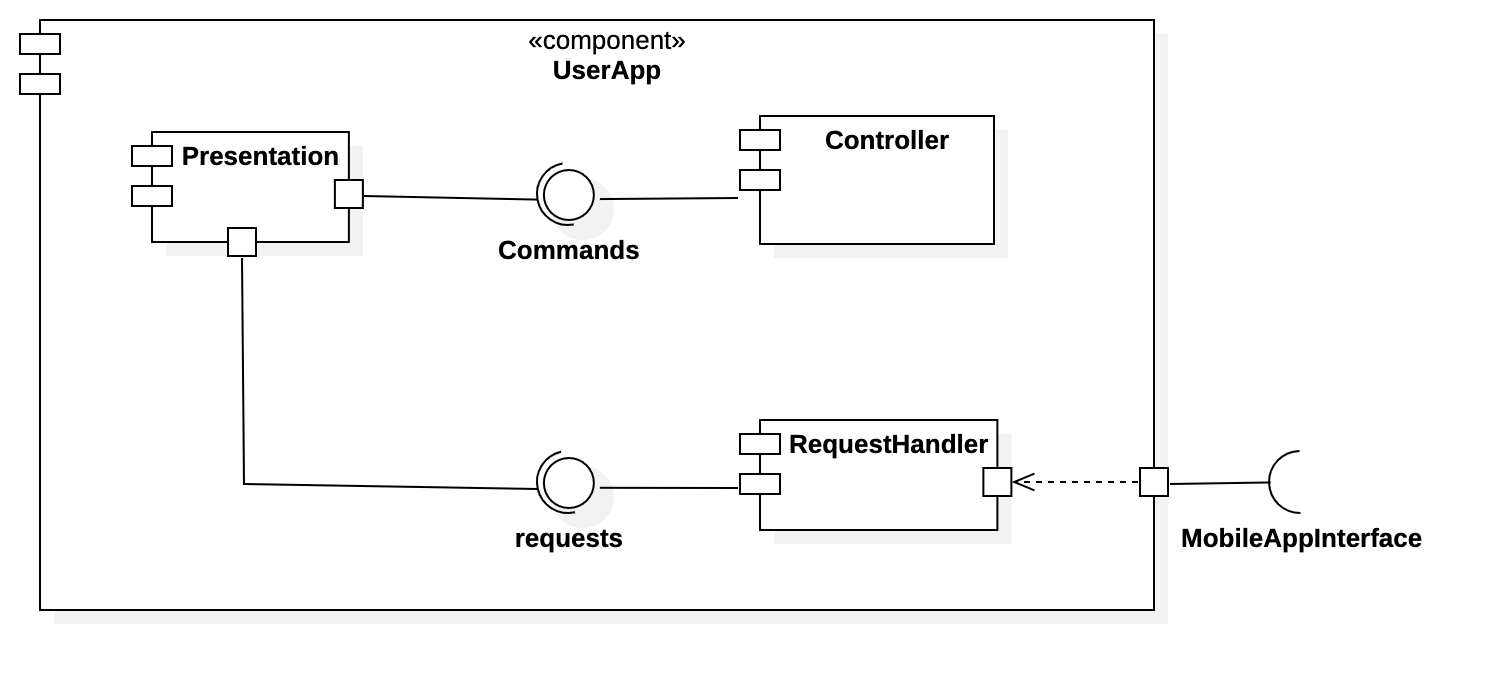
\includegraphics[scale=0.2]{/diagrams/components/userApp.png}
				\caption{\label{fig:userAppComp} User App Component Diagram}
			\end{figure}
		
	\subsection[Deployment View]{\hyperlink{toc}{Deployment View}}
		\label{sec:deploymentView}
		%todo implementations choices abbiamo la sezione apposta però ci stanno queste che metto
		
		\subsubsection[Decision Tree]{\hyperlink{toc}{Decision Tree}}
			\label{sec:decisionTree}
			
		\subsubsection[Deployment Diagram]{\hyperlink{toc}{Deployment Diagram}}
			\label{sec:deploymentDiagram}
			
	\subsection[Runtime View]{\hyperlink{toc}{Runtime View}}
		\label{sec:runtimeView}
		
	\subsection[Component Interfaces]{\hyperlink{toc}{Component Interfaces}}
		\label{sec:componentInterfaces}
		%todo all the APIs go here!
		
	\subsection[Selected Architectural Styles and Patterns]{\hyperlink{toc}{Selected Architectural Styles and Patterns}}
		\label{sec:selectedArchitecturalStylesAndPatterns}
		
	\subsection[Other Design Decisions]{\hyperlink{toc}{Other Design Decisions}}
		\label{sec:otherDesignDecisions}						